%%%%%%%%%%%%%%%%%%%%
% DESARROLLO DEL PROYECTO
%%%%%%%%%%%%%%%%%%%%

\section{Marco de Referencia}
\subsection{\'Areas Tem\'aticas}
\begin{itemize}
	\item Algoritmos computacionales.
	\item Almacenamiento en la nube.
	\item Bases de datos digitales.
	\item Ciencias agropecuarias. %agricolas? y pecuarias?
	\item Ganadería de carne.
	\item Ingeniería electrónica.
	\item Monitoreo digital.
	\item Sistemas RFID.
\end{itemize}

\subsection{Marco Te\'orico}

%Este proyecto consiste en el desarrollo de un sistema automático de bajo costo para el monitoreo de la alimentación de ganado involucrado en el ciclo productivo en la denominada "Ganadería de la Carne", es decir, reses que se encuentren en proceso de engorde o Ceba.
%El sistema podrá, mediante una variedad de sensores (peso, presencia y/o detección, tiempo real, RFID, comunicación vía Wifi), monitorear la alimentación respectiva de cada cabeza de ganado de forma particular e independiente de las demás mediante la toma y registro de datos en bases de datos en la nube. Esto se plantea mediante una propuesta electrónica basada en nuevas tecnologías y manejo de algoritmos computacionales.

%En este documento se propone un alimentador automático de bajo costo para reses en proceso de engorde o ceba que permita, mediante sensores de peso, suministrar una cantidad de alimento de manera automática para cada res, en horarios del día preestablecidos por el productor ganadero y cuya ración será respectiva al la dieta de cada animal basada en los intereses del propietario. Las reses estarían identificadas por un número ID colgando de sus cuerpos con lo cual se monitorea cada bovino por separado generando un historial alimenticio en la nube para cada individuo.
%Por medio de este alimentador se generaría un historial alimenticio de cada bovino que permitiría registrar la cantidad de porciones suministradas periódicamente, además de verificar, con sensores de presencia o detección,  si éste ha ingerido su alimento o no con lo cual se podrá identificar aquellas cabezas de ganado que estarían presentando desordenes alimenticios que vayan en contra de los intereses del productor.\\
%
%Entre los datos fijos de cada historial se tendría registro de su Nombre, RFID, Sexo, Raza, Peso y Edad inicial, Peso y Edad final; y como datos de monitoreo se tendría registro diario peso, edad, peso máximo alcanzado, si ha alcanzado o no un peso ideal y su evolución del peso para verificar si esta obteniendo un crecimiento positivo, o en caso contrario, proceder con la toma de decisiones respecto al sujeto en cuestión tales como su posible venta, tratamiento, o venta temprana, entre otros.
%
%Al estar identificados con un número ID propio e independiente, se ayuda se garantiza, mediante un sensor RFID, que el alimento se suministra al individuo correcto y que no se presentan casos en los que se suministren porciones repetidas en una misma franja horaria. Una vez el animal se encuentre en la zona de alimentación, estos serán pesados con el objetivo de hacer seguimiento del crecimiento de peso y verificar que esté cumpliendo con la rata de crecimiento fijada por el productor y en caso de alcanzar un peso máximo preestablecido o presentar disminución de peso hacer la respectiva notificación y observación en la nube para la toma de decisiones futuras.\\
%
%Por último el sistema verifica la cantidad neta de alimento suministrado y dará aviso preventivo, mediante un recordatorio o una alarma al personal encargado notificando si el alimento está próximo a acabarse.
%Es importante resaltar que este sistema se realiza con herramientas y sensores de bajo costo de Arduino.

%algoritmos que permitan obtener grandes cantidades de informaci\'on registrada en una base de datos para que esta información sirva como base para determinar tramos viales con mayor o menor deterioro vial. Esto se plantea mediante una propuesta electr\'onica basada en nuevas tecnolo\'ias y algoritmos computacionales.


\subsubsection{Alimentación}
La alimentación de un cultivo de ganado requiere de una dieta o ración con diferentes componentes básicos o nutrientes que deben ser suministrados día a día de forma balanceada para lograr un crecimiento óptimo y que los animales puedan expresar su potencial genético \cite{recomendaciones}. Los componentes principales que conforman la dieta alimenticia del ganado son:
	\begin{itemize}
	\item \textbf{Componentes básicos de la dieta} % Ponerle negrilla
		\begin{itemize}
		\item Agua: Componente principal de la alimentación. Esta debe ser suministrada en cantidad y calidad para ser aprovechada por cada animal llegando a ocupar mas del 50\% de la masa corporal de un ejemplar adulto y hasta un 90 \% de un recién nacido.
		\item Energía:  Este componente se suministra mediante azúcares, almidones, celulosa, entre otros, los cuales aportan grandes cantidades de energía mas no de proteína, razón por la cual se deben suministrar de forma complementaria.
		\item Proteínas: Estos nutrientes son fundamentales especialmente durantes los periodos de sequía para lo cual se optan por fuentes altas en proteína como leguminosas forrajeras como el Maní, Leucaena y el más común, los pastos de forraje verde. 
		\item Minerales: Son indispensables en la ganancia de peso de los novillos durante la etapa de Cría y Levante. Este complemento alimenticio debe estar siempre a la disposición para que el ganado pueda abastecer sus necesidades. Estos minerales se suelen proporcionar mediante mezclas de macrominerales y microminerales que se ofrecen de libre consumo al ganado.
		\item Vitaminas: Suministradas en cantidades pequeñas aplicadas comúnmente en animales cuya alimentación se basa en forrajes secos,  o en animales enfermos convalecientes, desnutridos o durante epocas de sequía prolongada.
		\end{itemize}
	\item \textbf{Balance de raciones y dietas especializadas} %Ponerle negrilla
Estas dietas son suministradas por personal técnico calificado que prepara un dieta acorde a la cantidad de nutrientes de cada animal de forma particular e independiente, considerando su peso actual, su velocidad de crecimiento y estado fisiológico.
	\end{itemize}
	
	
\subsubsection{Almacenamiento}
El alimento almacenado cae por gravedad al mecanismo de dosificación y este debe ser adaptado a su tamaño, densidad y peso \cite{pinturan}. Aparte del mecanismo, se debe tener en cuenta el material de contrucción, entre los materiales de fabricación mas comunes se encuentran el Poliestireno, Vidrio  y Céramica, Acero Inoxidable, Plástico,  entre otros. Estos deben garantizar resistencia y que cumpla con los requerimientos generales de almacenamiento de alimentos \cite{casti}:
\begin{itemize}
	\item El material de fabricación no debe modificar la composición, color, sabor, ni olor del producto contenido y no puede ceder componentes al medio interno ni externo que constituyan un riesgo para la salud.
	\item Fabricación con polímeros y aditivos que están incluidos en las listas positivas de las regulaciones alimentarias.
	\item Cumplir con los requisitos específicos de migración total en casos de compuestos químicos y componentes en el material plástico.
\end{itemize}


\subsubsection{Mecanismos de Dosificación}
El suministro de los alimentos del ganado cultivado se realiza mediante dispositivos electrónicos, mecánicos, electromecánicos y manuales. Estos dispositivos regulan el despacho del alimento en las diferentes etapas del cultivo de carne. A modo general, están compuestos por servomotores, motores eléctricos, cilindros neumáticos y/o reguladores electrónicos y mecánicos \cite{pinturan}. 
También pueden ser clasificados acorde a la naturaleza de la sustancia a manipular. Más propiamente dentro de la categoría de dosificadores volumetricos de sólidos secos, existen una gran variedad de mecanismos de dosificación  \cite{torres}, como algunos mencionados a continuación:

	\begin{itemize}
	
		\item \textbf{Dosificadores de Tornillo} % PONER NEGRILLA
		
		En estos dosificadores (Ver figura \ref{torni}) se tiene un Tornillo sin fin que actua como dosificador, éste se suele encontrar en la parte inferior de la tolva de alimentación y libera un volumen determinado de sustancia en cada vuelta; su velocidad y precisión de dosificación dependen de la velocidad de giro con la que se esté manipulando \cite{torres}. Este sistema de dosificación es el más utilizado debido a su implementación simple y porque se adapta a la naturaleza de la mayoría de las sustancias dosificadas.
		\begin{figure}[H]
			\begin{center}
				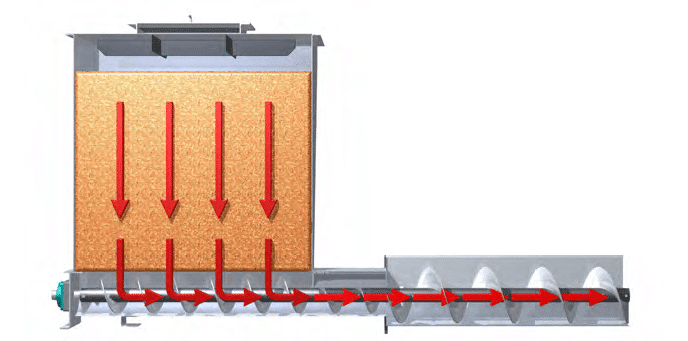
\includegraphics[scale=0.7]{img/tornillo.png}
			\end{center}
			\caption{Mecanismo de Tornillo sin fin. Tomada de \cite{DEM} \label{torni}}
		\end{figure} % Ponerle negrilla
		
		\item \textbf{Dosificadores de Compuerta Rotativa} % PONER NEGRILLA
		
		En este caso se tiene una compuerta rotativa como elemento principal de dosificación, permite una construcción simple y robusta, aunque presenta menor precisión que el mecanismo de tornillo sin fin. Una representación de este tipo de mecanismo se puede ver en la Figura \ref{rotala}.
		\begin{figure}[H]
			\begin{center}
				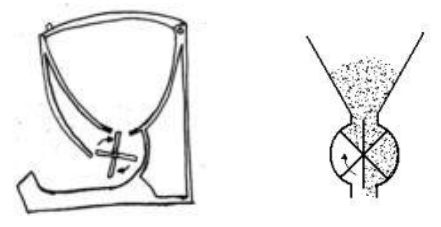
\includegraphics[scale=0.9]{img/rotar.png}
			\end{center}
			\caption{Mecanismo de Compuerta Rotativa. \label{rotala}}
		\end{figure} % Ponerle negrilla
		
		\item \textbf{Dosificadores de Compuerta deslizante} % PONER NEGRILLA
		
		Son compuertas deslizantes usadas para descargar material de tolvas, transportadores o compartimientos. La
compuerta deslizante consta de un marco rígido con una lámina deslizante ubicada en el interior que se abre y se cierra contra el flujo de material (Ver Figura \ref{deslis}). La placa deslizante puede ser accionada por medios manuales, neumáticos, eléctricos o hidráulicos. La lámina puede ser implementada de diferentes maneras y puede estar apoyada por rodamientos en 2 de sus extremos para facilitar la transición reduciendo así la fricción con las paredes del marco.
	
		\begin{figure}[H]
			\begin{center}
				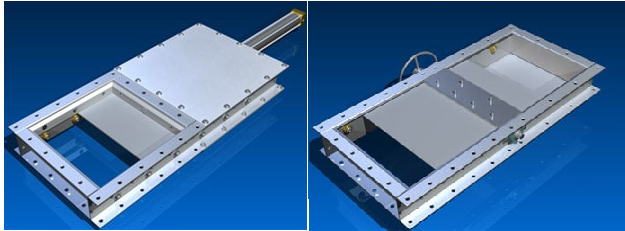
\includegraphics[scale=0.7]{img/slides.png}
			\end{center}
			\caption{Mecanismo de Compuerta Deslizante. Tomada de \cite{DEM} \label{deslis}}
		\end{figure} % Ponerle negrilla		
	\end{itemize}
	

\subsubsection{Leyes y Normatividad}  \label{leyes}
Requerida para que el avance ganadero se realice de manera coordinada o estandarizada basada en las buenas prácticas ganaderas en pro de mejorar la productividad y ayudarla a alcanzar niveles de ganadería bovina del mundo \cite{invima}. 
\begin{itemize}
	\item \textbf{Decreto 1500 de 2007:} Reglamento técnico a través del cual se crea el Sistema Oficial de Inspección, Vigilancia y Control de la Carne y otros productos comestibles y derivados cárnicos destinados para el consumo humano.
	\item \textbf{Decreto 072 de 2007:} Por el cual estable el manual de buenas prácticas de manejo para la producción de ganado bovino.
	\item \textbf{Decreto 2905 de 2007:} Por el cual se establece el reglamento técnico sobre los requisitos sanitarios y de inocuidad de la carne y productos cárnicos comestibles de las especies bovina y bufalina destinados para el consumo humano.
	\item \textbf{Decreto 18119 de 2007:} Por el cual se reglamenta los requisitos del plan gradual de cumplimiento para  las plantas de beneficio y desposte de bovino y bufalinos.
	\item \textbf{Decreto 2278 de 1982:} Reglamentación parcial en el titulo V de la ley 09 de 1979 que se refiere al sacrificio de animales de abasto público o para consumo humano y el procesamiento, transporte y comercialización de su carne.
\end{itemize}



\subsubsection{Conceptos adicionales}

\begin{itemize}

	\item \textbf{Algoritmos Computacionales:}
	Los algoritmos son un conjunto de instrucciones o reglas predefinidas de manera ordenada que permiten llevar a cabo una actividad mediante pasos consecutivos secuenciales o paralelos de manera no ambigua para poder realizar una actividad \cite{algoritmo}. Los algoritmos computacionales son algoritmos más sofisticados y precisos que permiten aprovechar las nuevas tecnolog\'ias y que al depender de una memoria finita deben ser lo mas optimizados posible para que puedan procesar grandes cantidades de datos con limitaciones finitas y generalmente a bajo costo. 

	\item \textbf{Almacenamiento en la nube:}
	 La nube, también denominada como ``Cloud Storage" (Ver Figura \ref{cloudpng}), se refiere tanto a las aplicaciones entregadas como servicios a través de internet y el sfotware del hardware y sistemas en los centros de datos que proporcionan estos servicios \cite{cloud2}.
	\begin{figure}[H]
	\begin{center}
		
\includegraphics[scale=0.35]{img/cloud.png}
	\end{center}
	\caption{Almacenamiento en nube. \label{cloudpng}}
	\end{figure}

	\item \textbf{Bases de datos digitales:}
	Es un conjunto de datos interrelacionados y almacenados de forma ordenada y sistem\'atica (Ver Figura \ref{databasepng}) para un uso posterior\cite{database}. Debido al desarrollo tecnol\'ogico de la inform\'atica y la electr\'onica, estas bases de datos suelen ser digitales y por lo general se almacenan en la nube (Cloud). Por otra parte, es considerado un modelo de almacenamiento de datos basado en redes de computadoras, donde los datos est\'an alojados en espacios de almacenamiento virtualizados \cite{cloud}.
	\begin{figure}[H]
		\begin{center}
			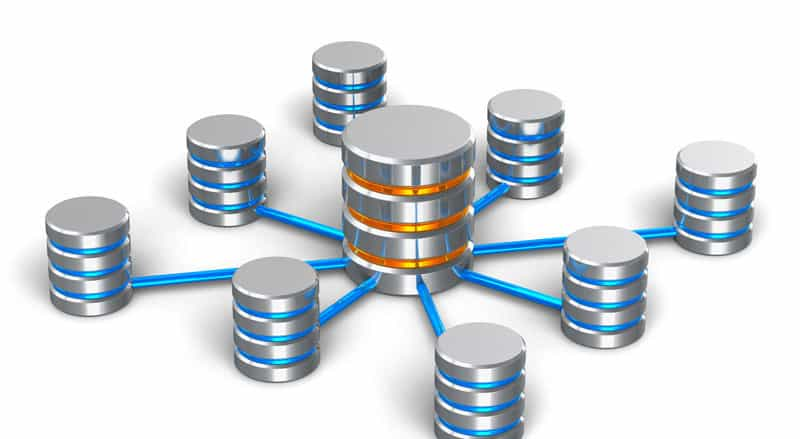
\includegraphics[scale=0.35]{img/databasepng.png}
		\end{center}
	\caption{Base de datos. \label{databasepng}}
	\end{figure}
	
	\item \textbf{Ganadería de carne:}
	 Es un ciclo productivo de cabezas de ganado destinadas al engorde que comprende un proceso prolongado en el tiempo que consta de varias etapas que abarcan desde el nacimiento vivo de la cría, siguiendo con su crecimiento y finalmente su comercialización en producto final, ya sea en carne, lácteos o sus derivados (Ver Figura \ref{ganadcarnepng}).
	 
	\begin{figure}[H]
	\begin{center}
		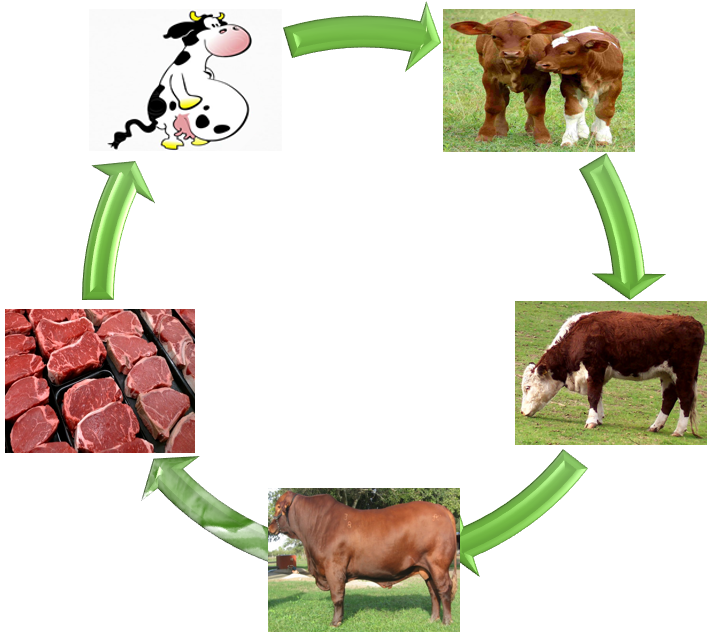
\includegraphics[scale=0.7]{img/ganadcarne.png}
	\end{center}
	\caption{Ganadería de carne. \label{ganadcarnepng}}
	\end{figure}
	
	\item \textbf{RFID:}
	 La identificación por radiofrecuencia (Ver Figura \ref{rfid1png}), es un sistema reprogramable de almacenamiento y recuperación de datos de manera inalámbrica mediante etiquetas, tarjetas o transpondedores en general, que pueden ser adheridas a productos, animales e incluso a personas sin necesidad de alimentación interna. Este sistema tiene una gran variedad de aplicaciones entre las cuales se pueden mencionar logísticas de distribución, servicios industriales, control de acceso, entre otros \cite{rfid1}.
	\begin{figure}[H]
	\begin{center}
		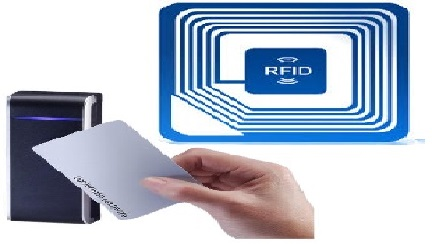
\includegraphics[scale=0.7]{img/rfid1.png}
	\end{center}
	\caption{Sistemas RFID. \label{rfid1png}}
	\end{figure}
	
\end{itemize}


%%%%%Debe incluir las referencias de manera adecuada, por ejemplo, \cite{cp-book}. (2-3 p\'aginas). Así mismo, los cuadros y figuras deben ser numeradas y referenciadas en el texto, por ejemplo, ver Figura \ref{escudo} y Cuadro \ref{tab:tabla-ejemplo}

%%%%%%%%%%%%%%%
% Figura de Ejemplo
%%%%%%%%%%%%%%%
%%\begin{figure}
%%	\begin{center}
%%		
\includegraphics{img/pujlogo.png}
%%	\end{center}
%%	\caption{Escudo Javeriana \label{escudo}}
%%\end{figure}

%%%%%%%%%%%%%%%
% Tabla de ejemplo
%%%%%%%%%%%%%%%

%%%\begin{table}
%%%\centering
%%%\begin{tabular}{ | l | l | l |}
%%%\hline
%%%{\bf Col 1} &{\bf  Col 2} & {\bf Col3} \\ \hline
%%%Fila 1 & Fila 2 & Fila 3 \\ \hline
%%%\end{tabular}
%%%\caption{Tabla de Ejemplo \label{tab:tabla-ejemplo}}
%%%\end{table}


\subsection{Trabajos Relacionados}
En esta área de trabajo se pueden encontrar innumerables trabajos de grado que usan al sector agroindustrial como oportunidad de desarrollo. Algunos de los trabajos previos y referentes al desarrollo de este trabajo de grado se pueden mencionar a los siguientes:

\begin{itemize}
\item \textbf{"Diseño, modelamiento y simulación de maquina dosificadora de alimento granulado para animales":} En este trabajo desarrollado por los estudiantes egresados de la Universidad de La Salle, Carlos Pinto y Hernán Durán, se puede  evidenciar el desarrollo tanto mecánico como electrónico de un dosificador giratorio de alimento granulada para aves.  El objetivo de este trabajo es facilitar el diseño de sistemas electrónicos que puedan ser implementados a nivel comercial, con la finalidad de  ayudar a incrementar el nivel productivo de las empresas ganaderas avícolas. En este proyecto se utilizó el modelamiento 3D como herramienta principal para el desarrollo del prototipo funcional usado para la dosificación del alimento granulado. El modelo final desarrollado se puede apreciar en la Figura \ref{lasal}:
			\begin{figure}[H]
			\begin{center}
			 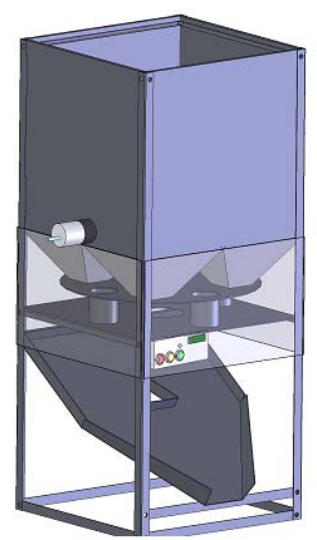
\includegraphics[scale=0.55]{img/lasal1png.png}
			\end{center}
			\caption{Unidad completa de dosificación. Tomada de \cite{pinturan} \label{lasal}}
			\end{figure}
			
\item \textbf{"Dispensador automático de comida para mascotas, programable y controlado remotamente":} Mediante este trabajado de grado, realizado por los Ingenieros Electrónicos de la Universidad del Valle John León y Daniel Rueda, se realiza el diseño y la implementación de un alimentador automático de mascotas que pueda ser controlador mediante una aplicación móvil para facilitar el uso y garantizar la dosificación del alimento al animal doméstico  en las horas que lo requiera \cite{univalle1}. Una característica similar al trabajo planteado es el uso de avisos y notificaciones móviles para los casos en los que el dispensador no cuente con suficiente alimento o que el dosificador no haya podido entregar el alimento correctamente.
Este sistema fue desarrollado mediante simulación e impresión 3D y la aplicación para la interfaz de usuario fue realizada mediante software Open Source para Android. El dispositivo final se puede apreciar en la Figura \ref{univalle1}:

			\begin{figure}[H]
			\begin{center}
			 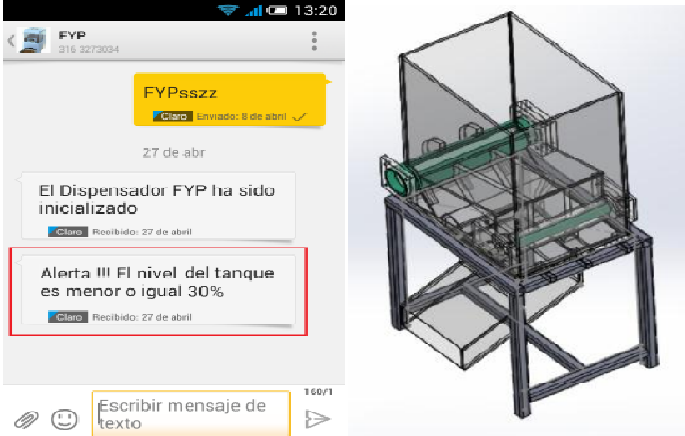
\includegraphics[scale=0.45]{img/univalle1png.png}
			\end{center}
			\caption{Unidad completa de dosificación. Tomada de \cite{univalle1} \label{univalle1}}
			\end{figure}			
			
\item \textbf{"Feedstar":} Este es un sistema automático de dosificación de alimento en grandes cantiadades especialmente diseñado para ahorrar espacio \cite{feedstar}. En la figura \ref{feedstar1} se observa una simulación del sistema, el cual puede ser regulado en tamaño y longitud y abastecer grandes cantidades de ganado mediante una correa extendible y un sistema de dosificación continuo que garantizan suministrar las grandes cantidades de alimento, minerales y forraje para abastecer ganado en sistemas de ganado estabulado. Este producto se encuentra a nivel comercial desarrollado por la empresa alemana EDER. 

			\begin{figure}[H]
			\begin{center}
			 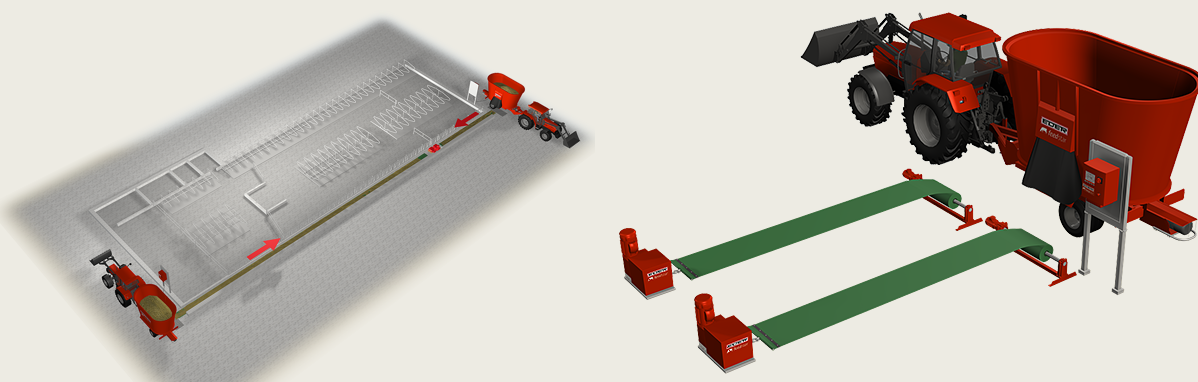
\includegraphics[scale=0.35]{img/feedstarpng.png}
			\end{center}
			\caption{Sistema Feedstar. Tomada de \cite{feedstar} \label{feedstar1}}
			\end{figure}	
			
			
\item \textbf{"Dosificador automático de alimento y agua para el ganado vacuno de la Finca Molina, en la comunidad de San Rafael del Sur":} Este es un trabajo de grado respaldado por la Universidad Autónoma de Nicaragua, que consiste en un sistema integral para suministrar alimento y agua a ganado vacuno en una finca de aproximadamente 7 hectáreas y el cual sería controlado mediante un PLC \cite{nicaraguat}. En este trabajo se plantea el diseño visto en la Figura \ref{nicaragua1} donde se puede observar el control de diferentes sensores para proveer correcta y eficientemente la dosificación de alimento y agua por cada cabeza de ganado ubicadas en sus respectivos cubículos perteneciente al sistema.

			\begin{figure}[H]
			\begin{center}
			 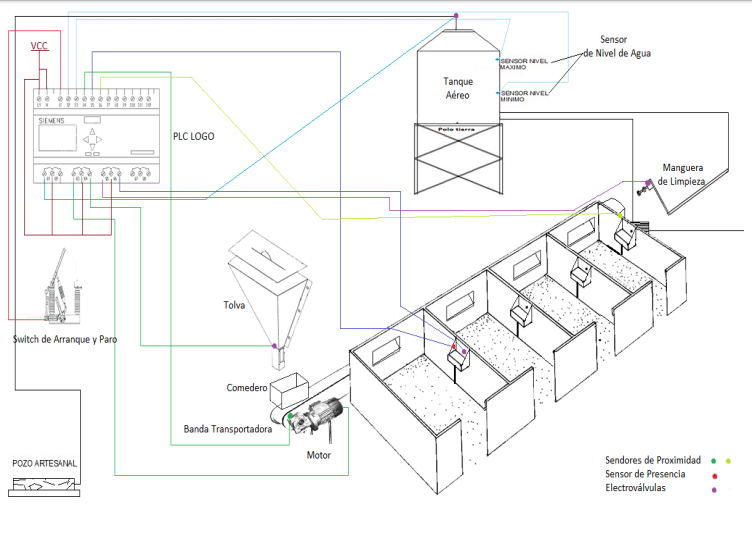
\includegraphics[scale=0.9]{img/nicaraguapng.png}
			\end{center}
			\caption{Sistema alimenticio de la Finca Molina. Tomada de \cite{nicaraguat} \label{nicaragua1}}
			\end{figure}	
			
			
\end{itemize}


\section{Metodolog\'ia}

\subsection{Tipo de Estudio y Metodolog\'ia a usar} 
%Definir y explicar el tipo de estudio (exploratorio, descriptivo, correlacional, explicativo).
Este proyecto, al igual que todo proceso de desarrollo, tiene un m\'etodo que caracteriza su evoluci\'on; por tal raz\'on se propone el uso de la metodolog\'ia CDIO como base metodol\'ogica para la realizaci\'on de este proyecto. 
Esta metodología  ha sido formada por las principales escuelas de Ingeniería de Estados Unidos, Europa, Canadá, Reino Unido, África, Asia y Nueva Zelanda; como una forma de colaboración a nivel mundial para desarrollar una nueva visión de enseñanza de la ingeniería.\\

Esta metodolog\'ia permite proporcionar las herramientas necesarias para desarrollar propuestas innovadoras a trav\'es de un an\'alisis sistem\'atico a partir de la problem\'atica planteada. y est\'a compuesta por 4 fases que consisten en Concebir, Diseñar, Implementar y Operar sistemas de ingeniería con valor agregado en un ambiente moderno para crear sistemas y productos. El proyecto ser\'a  dirigido y monitoreado por parte del director del proyecto semanalmente para verificar, controlar y corregir lo que se irá trabajando día a día por el estudiante a lo largo del proyecto.

\begin{itemize}
	\item \textbf{NOTA 1: Debido a los alcances mencionados en la secci\'on \ref{limites}, este proyecto no incluir\'a la fase de Implementaci\'on debido a que este es un proyecto de dise\~no. Mas sin embargo constará de una construcción de un prototipo para suplir la fase de Implementación y validar la fase de Operación.}
	\item \textbf{NOTA 2: La realizaci\'on de tareas no necesariamente es de manera secuencial y se encontrar\'an actividades que se realicen paralelamente}.\\\\
\end{itemize}

\subsection{Actividades} \label{actividades}
%\textbf{\textit{\Estas todavía no son las actividades es solo como para ver como quedaría una estructura parecida, ES soo un FORMATO}}
\begin{itemize}
\item[1)] Fase de Concepción:
	\begin{itemize}
	
	\item Identificaci\'on del área temática, normatividad, limitaciones técnicas y tecnológicas, usuarios; contextos sociales, culturales, ambientales y necesidades de la problem\'atica.
	\item Búsqueda bibliogr\'afica referente a la tem\'atica.
	\item Analizar trabajos previos y antecedentes para búsqueda de oportunidades o posibles mejoras.
	\item Investigaci\'on de posibles herramientas y dispositivos que aporten al desarrollo del trabajo de grado.
	\item Buscar, clasificar y seleccionar las herramientas y los dispositivos a utilizar.
	\item Establecer parámetros de entrada y salida (In/Out).

	\end{itemize}
	
\item[2)] Fase de Dise\~no:
	\begin{itemize}

	\item Dise\~nar el sistema de medici\'on y obtenci\'on de informaci\'on.
	\item Dise\~nar los algoritmos para cada dispositivo con base en los parámetros In/Out.
	\item Dise\~nar la identificación exitosa de cada animal por separado.
	\item Dise\~nar la verificación de alimento suficiente para dar abasto a las raciones del día.
	\item Dise\~nar el aviso o alarma en caso que no haya suficiente alimento para suplir las necesidades dietarias del día para los animales.
	\item Dise\~nar la dosificación del alimento y los mecanismos que se requieran para tal fin.
	\item Dise\~nar el pesaje de la ración dosificada que será suministrada a cada res de acuerdo con su dieta respectiva.
	\item Dise\~nar el suministro del alimento dosificado.
	\item Dise\~nar la verificación de que el alimento ha sido suministrado.
	\item Dise\~nar la verificación de que el alimento suministrado ha sido ingerido satisfactoriamente.
	\item Dise\~nar la verificación que permita corroborar si un animal ya ha sido alimentado en una franja horaria determinada para negar dosificaciones repetidas.
	\item Dise\~nar el aviso o la alarma en caso de presentarse un caso de negación por dosificación repetida.
	\item Dise\~nar el aviso al personal y registro en el historial de la res correspondiente en caso tal que no se ingiera el alimento
	\item Dise\~nar el proceso para la toma de peso de cada una de las reses en un grupo determinado. 
	\item Dise\~nar el registro de la información de manera automática.
	\item Dise\~nar la representaci\'on de la informaci\'on.
	\item Dise\~nar el prototipo del prototipo a escala para la prueba del concepto.
	\item Dise\~nar el plan de pruebas.
	
	\end{itemize}
	
\item[3)] Fase de Construcci\'on:

	\begin{itemize}
	
	\item Construcción del prototipo.
	\item Construcción del plan de pruebas.
	
	\end{itemize}
	
\item[4)] Fase de Operaci\'on:

	\begin{itemize}
	
	\item Verificaci\'on de la funcionalidad de los dispositivos.
	\item Verificaci\'on de la funcionalidad de los algoritmos.
	\item Verificación de los resultados para correcciones (si la hay) del plan de pruebas.
	\item Verificaci\'on de la funcionalidad del prototipo.
	\item Evaluaci\'on de los resultados.
	
	\end{itemize}

\item[5)] Otros:

	\begin{itemize}
	
	\item Reuniones de control con director del proyecto.
	\item Realización de la documentación del proyecto.
	
	\end{itemize}
\end{itemize}		

\section{Resultados Esperados}
% Hip\'otesis que se deben evaluar al final del proyecto (1 p\'agina)\\
 
 Los resultados esperados en este proyecto son:
 \begin{itemize}
 	\item Diseño de un sistema automático de alimentación de ganado de reses estabuladas en proceso de Ceba.
 	\item Identificar a cada individuo por separado mediante el sensor de RFID.
 	\item Dosificar exitosamente raciones de un gramaje acorde a la porción requerida para cada animal cultivado basado en su dieta preestablecida.
 	\item Tomar registro de la dosificación y entrega exitosa de alimento.
 	\item Verificar la cantidad de alimento racionado antes de ser depositado en la bandeja y tomar registro de ello.
 	\item Entregar el alimento racionado a cada individuo una única vez en una misma franja horaria y tomar registro de ello.
 	\item Dar aviso si se presenta un caso de intento de repetición de ración dosificada en una misma franja horaria por un mismo animal.
 	\item Verificar que el animal haya ingerido su porción, tomar registro de ello y dar aviso en caso contrario. 	
 	\item Obtener el peso del animal y tomar registro de ello.
 	\item Verificar que se tenga alimento suficiente para suministrar las porciones del día y dar aviso oportuno en caso contrario.
 	\item Hacer registro en la nube de los datos registrados por cada sensor.
 	\item Dar aviso de observaciones predefinidas por el productor de ceba mediante avisos y/o alarmas.
 	\item Mostrar los datos evolutivamente mediante ayudas gráficas.
 	\item Prototipo físico (a escala) del sistema diseñado con un solo dosificador funcional.
 	\item El diseño del prototipo y del sistema total posibilite hasta 4 dosificadores completamente funcionales.
 	\item Plan de pruebas.%\\ \\ \\ \\ \\ \\ \\ \\ \\ \\ \\ \\ \\ \\ \\ \\ \\ \\ \\ \\ \\ \\ \\ \\ \\ \\    
 \end{itemize} 
% 
\section{Cronograma}
%%%El cronograma por semana incluyendo las actividades descritas en la Secci\'on \ref{actividades}. 
En el Cuadro \ref{cronograma}, se evidencian las actividades previamente mencionadas en la sección \ref{actividades}, las cuales se realizar\'an para el desarrollo del proyecto.
%\\ \\ \\ \\ \\
% \ref{cronograma}.
 
%%%\begin{table}[H]
%%%	\begin{center}
%%%		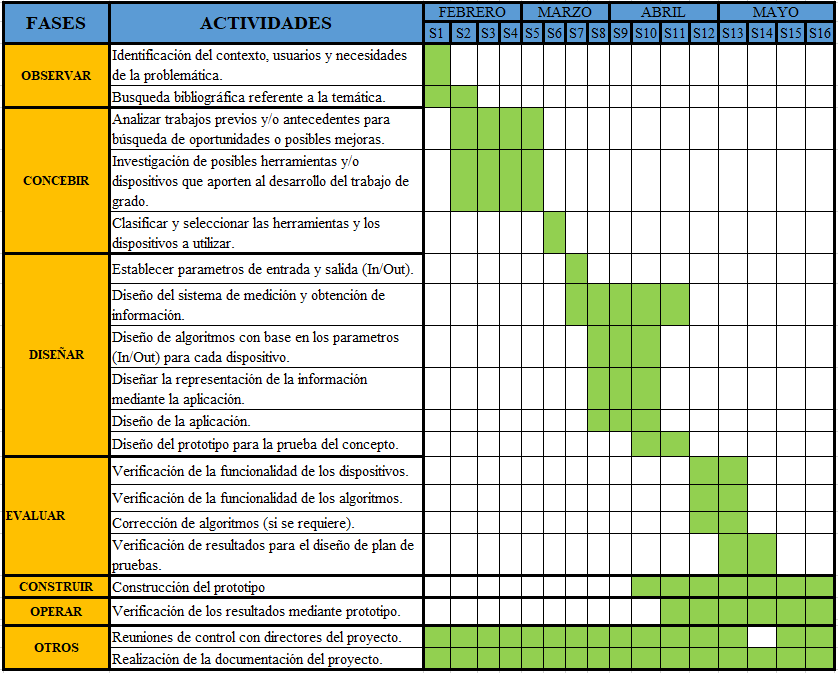
\includegraphics[scale=0.8]{img/cronopng4_5.png} %este comienzxa en febrero por als correciones de alexander
%%%	\end{center}
%%%	\caption{Cronograma del proyecto. \label{cronograma}}
%%%\end{table}
\begin{table}%[H]

\begin{ganttchart}[ 
x unit = 0.22cm, 
y unit chart = 0.4 cm,
y unit title = 0.45 cm,
milestone label font=\tiny,
group label font=\small,
title label font=\tiny,
%bar label font=\tiny,
time slot format=isodate, 
time slot format/start date=2015-03-25,
progress=today,
%time slot unit=week,
%canvas/.append style={fill=none, draw=black!60 , line width=.75pt},  %Este es el cuadrado blanco "La hoja" por así decrilo donde estan las barras del diagrama de gantt, esta sin fill y con bordes (yo creo que un 60 eta bien) y el grosor esta bien
hgrid,% style/.style={draw=none, line width=0pt}, % Esta es una linea que esta debajo del titulo  (Cronograma de actividades en este caso)
vgrid,%={*1{draw=black!40, line width=.5pt}}, % Estas son las lineas verticales del Diagrama de gantt, es mejor dejarlas delgadas y claras
%today=1,%\today,
today={\the\year-\the\month-\the\day},
today rule/.style={draw=black!90,dash pattern=on 3.0pt off 4.5pt,line width=1.2pt},
today label font=\small\bfseries,
%title/.style={draw=none, fill=none},%%%%%%%%%%%%%%%%%%%%%%%%%%%%%%%%%%%%%%%%%%%%%%%%%%%%%%%%%%%
%%%title label font=\bfseries\footnotesize,
%%%title label node/.append style={below=0pt}, % esto es que tan separado del titulo estan Marzo, Abril y Mayo
%%%include title in canvas=true, % hace llegar el recuadro de la cuadricula hasta por encima del titulo y se veo feo SI ESTA EN TRUE
bar label font=\mdseries\tiny\color{black!85}, % esto afecta la tonalidad de las palabras ACTIVIDAD 1.2.3.....
%%%%%bar label node/.append style={align=left,left=1cm}, % Separación entre las actividades y la cuadricula con las barras de gantt
bar label node/.append style={left=0.1cm},
bar/.append style={draw=none, fill=bargreen}, % ESTE NUMERO CAMBIA LA TONALIDAD DEL LA BARRA que va completando la tarea
%  EN UN PORCENTAJE DE NEGRO DEL 1-100
bar incomplete/.append style={fill=barblue}, % cambia la barra de fondo que es la que se debe completar en el porcentaje de avance
bar progress label font=\mdseries\tiny\color{black!99}, % Cambia la tonalidad del Porcentaje -> ejemplo ==== 10% completado
bar progress label node/.append style={below left=-6pt and -33pt},
bar label node/.append style={below left=-7pt and 0pt},%que tan hacia arriba o abajo aparece el letrero Activity
%%% de Finish to start y que tan hacia la derecha o izquierda aparece
group incomplete/.append style={fill=black!15}, % esta es la barra  del avance total del cronograma
group progress label font=\mdseries\small\color{black!99}, %footnotesize
group progress label node/.append style={below left=-6pt and -33pt},
group label node/.append style={below left=6pt and 0pt},
%%group left shift=0,
%%group right shift=0,
group height=0.4, % Esto es que tan alta es la barra grande del avance neto del proyecto
group peaks tip position=0,
group label node/.append style={left=0.1cm},
group/.append style={draw=none, fill=groupgreen}, % ESTE NUMERO CAMBIA LA TONALIDAD DEL LA BARRA que va completando la tarea
group progress label font=\bfseries\tiny,
%%link/.style={-latex, line width=1.5pt, linkred},
%%link label font=\scriptsize\bfseries,
%%link label node/.append style={below left=-2pt and 0pt},%que tan hacia arriba o abajo aparece el letrero
%%% de Finish to start y que tan hacia la derecha o izquierda aparece
]
%{1}{10}
{2019-03-25}{2019-05-30}
%{2019/03/25}{2019/05/30}
%\gantttitlecalendar{year, month=shortname, week, day} \\
\gantttitlecalendar{year, month=name, week} \\
%\gantttitlecalendar*[compress calendar,time slot format=isodate]{2019-03-22}{2019-05-30}{year, month} \\
%\gantttitlecalendar*[compress calendar,time slot format=isodate]{2015-11-1}{2018-10-30}{year, month} \\


%\ganttbar[bar/.append style={fill=blue}]{Goal Document}{2015-03-02}{2015-03-20}\\ 

%%%%\gantttitle{CRONOGRAMA DE ACTIVIDADES}{10} \\[grid]
%\gantttitle{CRONOGRAMA DE ACTIVIDADES}{10} \\[grid]
%\gantttitle{Marzo}{2}
%\gantttitle{Abril}{4}
%\gantttitle{Mayo}{4}\\
%\gantttitle[title label node/.append style={below left=-1pt and 15pt}]{Semana N.o:}{0} 
% Esto es la posicion hacia abajo de lo que dice Semana N.o 1
%\gantttitlelist{1,...,10}{1} \\

\ganttgroup{THESIS}{2019-03-25}{2019-05-30} \\
%\ganttgroup{THESIS}{2019/03/25}{2019/05/30} \\
%\ganttgroup[progress=20]{TESIS}{1}{10} \\
%%%
\ganttgroup{CONCEIVE}{2019-03-25}{2019-05-03} \\
%\ganttgroup{CONCEIVE}{2019/03/25}{2019/05/03} \\
%%%\ganttgroup[progress=65]{CONCEBIR}{1}{6} \\
%%%
\ganttbar[name=bar1]{\textbf{Activity 1}}{2019-03-25}{2019-03-30} \\
%\ganttbar[name=bar1]{\textbf{Activity 1}}{2019/03/25}{2019/03/30} \\
%%%\ganttbar[progress=100,name=bar1]{\textbf{Activity 1}}{1}{1} \\
%%%
\ganttbar[name=bar2]{\textbf{Activity 2}}{2019-03-25}{2019-03-30} \\
%\ganttbar[name=bar2]{\textbf{Activity 2}}{2019/03/25}{2019/03/30} \\
%%%\ganttbar[progress=14,name=bar2]{\textbf{Activity 2}}{1}{1} \\
%%%
\ganttbar[name=bar3]{\textbf{Activity 3}}{2019-03-25}{2019-03-30} \\
%\ganttbar[name=bar3]{\textbf{Activity 3}}{2019/03/25}{2019/03/30} \\
%%%\ganttbar[progress=25,name=bar3]{\textbf{Activity 3}}{1}{1} \\
%%%
\ganttbar[name=bar4]{Activity 4}{2019-03-25}{2019-03-30} \\
%\ganttbar[name=bar4]{Activity 4}{2019/03/25}{2019/03/30} \\

%%%\ganttbar[progress=56,name=bar4]{Activity 4}{1}{1} \\
%%%
\ganttbar[name=bar5]{\textbf{Activity 5}}{2019-03-25}{2019-04-30} \\
%\ganttbar[name=bar5]{\textbf{Activity 5}}{2019/03/25}{2019/04/30} \\
%%%\ganttbar[progress=100,name=bar5]{\textbf{Activity 5}}{1}{6} \\
%%%
\ganttbar[name=bar6]{\textbf{Activity 6}}{2019-03-25}{2019-04-30} \\
%\ganttbar[name=bar6]{\textbf{Activity 6}}{2019/03/25}{2019/04/30} \\
%%%\ganttbar[progress=100,name=bar6]{\textbf{Activity 6}}{1}{6} \\
%%%
\ganttgroup{DESIGN}{2019-04-01}{2019-05-18} \\
%\ganttgroup{DESIGN}{2019/04/01}{2019/05/18} \\
%%%\ganttgroup[progress=30]{DISEÑAR}{2}{8} \\
%%%
\ganttbar[name=bar7]{\textbf{Activity 7}}{2019-04-01}{2019-05-05} \\
%\ganttbar[name=bar7]{\textbf{Activity 7}}{2019/04/01}{2019/05/05} \\
%%%\ganttbar[progress=14,name=bar7]{\textbf{Activity 7}}{2}{6} \\
%%%
\ganttbar[name=bar8]{\textbf{Activity 8}}{2019-04-01}{2019-05-05} \\
%\ganttbar[name=bar8]{\textbf{Activity 8}}{2019/04/01}{2019/05/05} \\
%%%\ganttbar[progress=25,name=bar8]{\textbf{Activity 8}}{2}{6} \\
%%%
\ganttbar[name=bar9]{\textbf{Activity 9}}{2019-04-01}{2019-04-14} \\
%\ganttbar[name=bar9]{\textbf{Activity 9}}{2019/04/01}{2019/04/14} \\
%%%\ganttbar[progress=56,name=bar9]{\textbf{Activity 9}}{2}{3} \\
%%%
\ganttbar[name=bar10]{\textbf{Activity 10}}{2019-04-01}{2019-04-14} \\
%\ganttbar[name=bar10]{\textbf{Activity 10}}{2019/04/01}{2019/04/14} \\
%%%\ganttbar[progress=100,name=bar10]{\textbf{Activity 10}}{2}{3} \\
%%%
\ganttbar[name=bar11]{\textbf{Activity 11}}{2019-04-01}{2019-04-21} \\
%\ganttbar[name=bar11]{\textbf{Activity 11}}{2019/04/01}{2019/04/21} \\
%%%\ganttbar[progress=100,name=bar11]{\textbf{Activity 11}}{2}{4} \\
%%%
\ganttbar[name=bar12]{\textbf{Activity 12}}{2019-04-01}{2019-04-21} \\
%\ganttbar[name=bar12]{\textbf{Activity 12}}{2019/04/01}{2019/04/21} \\
%%%\ganttbar[progress=14,name=bar12]{\textbf{Activity 12}}{2}{4} \\
%%%
\ganttbar[name=bar13]{\textbf{Activity 13}}{2019-04-08}{2019-04-14} \\
%\ganttbar[name=bar13]{\textbf{Activity 13}}{2019/04/08}{2019/04/14} \\
%%%\ganttbar[progress=25,name=bar13]{\textbf{Activity 13}}{3}{3} \\
%%%
\ganttbar[name=bar14]{\textbf{Activity 14}}{2019-04-15}{2019-04-21} \\
%\ganttbar[name=bar14]{\textbf{Activity 14}}{2019/04/15}{2019/04/21} \\
%%%\ganttbar[progress=56,name=bar14]{\textbf{Activity 14}}{4}{4} \\
%%%
\ganttbar[name=bar15]{\textbf{Activity 15}}{2019-04-15}{2019-04-21} \\
%\ganttbar[name=bar15]{\textbf{Activity 15}}{2019/04/15}{2019/04/21} \\
%%%\ganttbar[progress=20,name=bar15]{\textbf{Activity 15}}{4}{4} \\
%%%
\ganttbar[name=bar16]{\textbf{Activity 16}}{2019-04-15}{2019-04-21} \\
%\ganttbar[name=bar16]{\textbf{Activity 16}}{2019/04/15}{2019/04/21} \\
%%%\ganttbar[progress=30,name=bar16]{\textbf{Activity 16}}{4}{4} \\
%%%
\ganttbar[name=bar17]{\textbf{Activity 17}}{2019-04-01}{2019-04-14} \\
%\ganttbar[name=bar17]{\textbf{Activity 17}}{2019/04/01}{2019/04/14} \\
%%%\ganttbar[progress=14,name=bar17]{\textbf{Activity 17}}{2}{3} \\
%%%
\ganttbar[name=bar18]{\textbf{Activity 18}}{2019-04-01}{2019-04-21} \\
%\ganttbar[name=bar18]{\textbf{Activity 18}}{2019/04/01}{2019/04/21} \\
%%%\ganttbar[progress=25,name=bar18]{\textbf{Activity 18}}{2}{4} \\
%%%
\ganttbar[name=bar19]{\textbf{Activity 19}}{2019-04-01}{2019-04-21} \\
%\ganttbar[name=bar19]{\textbf{Activity 19}}{2019/04/01}{2019/04/21} \\
%%%\ganttbar[progress=56,name=bar19]{\textbf{Activity 19}}{2}{4} \\
%%%
\ganttbar[name=bar20]{\textbf{Activity 20}}{2019-04-08}{2019-04-28} \\
%\ganttbar[name=bar20]{\textbf{Activity 20}}{2019/04/08}{2019/04/28} \\
%%%\ganttbar[progress=20,name=bar20]{\textbf{Activity 20}}{3}{5} \\
%%%
\ganttbar[name=bar21]{\textbf{Activity 21}}{2019-04-08}{2019-05-5} \\
%\ganttbar[name=bar21]{\textbf{Activity 21}}{2019/04/08}{2019/05/5} \\
%%%\ganttbar[progress=10,name=bar21]{\textbf{Activity 21}}{3}{6} \\
%%%
\ganttbar[name=bar22]{\textbf{Activity 22}}{2019-04-22}{2019-05-12} \\
%\ganttbar[name=bar22]{\textbf{Activity 22}}{2019/04/22}{2019/05/12} \\
%%%\ganttbar[progress=14,name=bar22]{\textbf{Activity 22}}{5}{7} \\
%%%
\ganttbar[name=bar23]{\textbf{Activity 23}}{2019-04-15}{2019-05-12} \\
%\ganttbar[name=bar23]{\textbf{Activity 23}}{2019/04/15}{2019/05/12} \\
%%%\ganttbar[progress=25,name=bar23]{\textbf{Activity 23}}{4}{7} \\
%%%
\ganttbar[name=bar24]{\textbf{Activity 24}}{2019-04-01}{2019-05-19} \\
%\ganttbar[name=bar24]{\textbf{Activity 24}}{2019/04/01}{2019/05/19} \\
%%%\ganttbar[progress=56,name=bar24]{\textbf{Activity 24}}{2}{8} \\
%%%
\ganttgroup{CONSTRUCT}{2019-04-1}{2019-05-19} \\
%\ganttgroup{CONSTRUCT}{2019/04/1}{2019/05/19} \\
%%%\ganttgroup[progress=30]{CONSTRUIR}{2}{8} \\
%%%
\ganttbar[name=bar25]{\textbf{Activity 25}}{2019-04-22}{2019-05-19} \\
%\ganttbar[name=bar25]{\textbf{Activity 25}}{2019/04/22}{2019/05/19} \\
%%%\ganttbar[progress=10,name=bar25]{\textbf{Activity 25}}{5}{8} \\
%%%
\ganttbar[name=bar26]{\textbf{Activity 26}}{2019-04-22}{2019-05-19} \\
%\ganttbar[name=bar26]{\textbf{Activity 26}}{2019/04/22}{2019/05/19} \\
%%%\ganttbar[progress=10,name=bar26]{\textbf{Activity 26}}{5}{8} \\
%%%
\ganttgroup{OPERATE}{2019-04-15}{2019-05-30} \\
%\ganttgroup{OPERATE}{2019/04/15}{2019/05/30} \\
%%%\ganttgroup[progress=30]{OPERAR}{4}{10} \\
%%%
\ganttbar[name=bar27]{\textbf{Activity 27}}{2019-05-06}{2019-05-26} \\
%\ganttbar[name=bar27]{\textbf{Activity 27}}{2019/05/06}{2019/05/26} \\
%%%\ganttbar[progress=14,name=bar27]{\textbf{Activity 27}}{7}{9} \\
%%%
\ganttbar[name=bar28]{\textbf{Activity 28}}{2019-05-06}{2019-05-26} \\
%\ganttbar[name=bar28]{\textbf{Activity 28}}{2019/0506}{2019/05/26} \\
%%%\ganttbar[progress=25,name=bar28]{\textbf{Activity 28}}{7}{9} \\
%%%
\ganttbar[name=bar29]{\textbf{Activity 29}}{2019-05-06}{2019-05-26} \\
%\ganttbar[name=bar29]{\textbf{Activity 29}}{2019/05/06}{2019/05/26} \\
%%%\ganttbar[progress=56,name=bar29]{\textbf{Activity 29}}{7}{9} \\
%%%
\ganttbar[name=bar30]{\textbf{Activity 30}}{2019-05-13}{2019-05-30} \\
%\ganttbar[name=bar30]{\textbf{Activity 30}}{2019/05/13}{2019/05/30} \\
%%%\ganttbar[progress=56,name=bar30]{\textbf{Activity 30}}{8}{9.5} \\
%%%
\ganttbar[name=bar31]{\textbf{Activity 31}}{2019-05-13}{2019-05-30} \\
%\ganttbar[name=bar31]{\textbf{Activity 31}}{2019/05/13}{2019/05/30} \\
%%%\ganttbar[progress=56,name=bar31]{\textbf{Activity 31}}{8}{10} \\
%%%
\ganttgroup{OTHERS}{2019-03-25}{2019-05-30} \\
%\ganttgroup{OTHERS}{2019-03-25}{2019-05-30} \\
%%%\ganttgroup[progress=30]{OTROS}{1}{10} \\
%%%
\ganttbar[name=bar32]{\textbf{Activity 32}}{2019-03-25}{2019-05-30} \\
%\ganttbar[name=bar32]{\textbf{Activity 32}}{2019/03/25}{2019/05/30} \\
%%%\ganttbar[progress=56,name=bar32]{\textbf{Activity 32}}{1}{10} \\
%%%
\ganttbar[name=bar33]{\textbf{Activity 33}}{2019-03-25}{2019-05-30}
%\ganttbar[name=bar33]{\textbf{Activity 33}}{2019/03/25}{2019/05/30}
%%%\ganttbar[progress=56,name=bar33]{\textbf{Activity 33}}{1}{10} \\
%

%\ganttmilestone{Hito 1}{11}{11}  \\
%\ganttmilestone{Hito 2}{12}{12} \\
%\ganttbar[progress=35,]{\textbf{Activity 8}}{12}{22} \\
%\ganttbar[progress=0,]{\textbf{Activity 9}}{23}{24} \\
%\ganttmilestone{Q6 report}{9}{10} \\
%\ganttmilestone{M2: Project finished}{5}{10}


%%%\ganttlink[link type=f-s]{bar1}{bar2}
%%%\ganttlink[link type=f-s]{bar4}{bar5}


\end{ganttchart}
\caption{Cronograma del proyecto. \label{cronograma}}
\end{table}
%\end{tikzpicture}


%\end{document}


\section{Recursos}

\subsection{Humanos}
\subsubsection{Director}
\begin{itemize}
\item El ingeniero Electr\'onico, Eugenio Tamura. Curs\'o su pregrado en la Universidad del Cauca.
Obtuvo su Maestr\'ia y Doctorado en Arquitectura y Tecnolog\'ia de los Sistemas Inform\'aticos, en la Universidad Polit\'ecnica de Valencia, Espa\~na.\\
Actualmente es Director de Carrera de Ingenier\'ia Electr\'onica  y profesor de Pregrado, Maestr\'ia y Doctorado.

\end{itemize} 
\subsubsection{Estudiante}
El estudiante de Ingenier\'ia Electr\'onica  \authorA, llevar\'a a cabo el desarrollo de este proyecto para optar por el título de Ingeniero Electrónico en la Pontificia Universidad Javeriana Cali.


%%%%%%%%%%%%%%%
% Tabla de ejemplo
%%%%%%%%%%%%%%%

%%%\begin{table}
%%%\centering
%%%\begin{tabular}{ | l | l | l |}
%%%\hline
%%%{\bf Col 1} &{\bf  Col 2} & {\bf Col3} \\ \hline
%%%Fila 1 & Fila 2 & Fila 3 \\ \hline
%%%\end{tabular}
%%%\caption{Tabla de Ejemplo \label{tab:tabla-ejemplo}}
%%%\end{table}


\subsection{Econ\'omicos}
\subsubsection{Consideraciones}
El desarrollo de este proyecto requerir\'a establecer lo siguiente:


\begin{itemize}

	\item Consideraciones del proyecto respecto a la Universidad visto en el cuadro \ref{tabconsidPUJ}:
	
\begin{table}[H]
\centering
\scalebox{0.8}{
{\setlength{\arrayrulewidth}{0.8mm}
\begin{tabular}{ | >{\columncolor{tabla1}} p{3.8cm} | p{0.45cm} | >{\columncolor{tabla1}} p{3.0cm} | p{2.1cm} | >{\columncolor{tabla1}} p{3.5cm} | p{4cm} | }
\hline
{\bf\centering \bfseries\small Director(es)} & {\bf\centering  1} & {\bf\centering \bfseries\small Salario Mensual por Director \\ (Aproximado).}
 & {\bf\centering \bfseries\small \$ 7'.000.000} & {\bf\centering \bfseries\small Cantidad total de horas por  semana} & {\bf\centering  2}\\ \hline
{\bf\centering \bfseries\small \# Días trabajados al mes} & {\bf\centering   20} & {\bf\centering \bfseries\small Horas trabajadas al día} & {\bf\centering   8}
 & {\bf\centering \bfseries\small  Frecuencia de atención y dirección (semanal)} & {\bf\centering  1-2}\\ \hline
{\bf\centering \bfseries\small \# Horas de dirección por sesión } & {\bf\centering  2.5} & {\bf\centering \bfseries\small Costo Hora Director} & {\bf \bfseries\small \$ 43.750} & {\bf\centering \bfseries\small  Equipos de trabajo} & {\bf\centering  \bfseries\small Propios de la Universidad}\\ \hline
{\bf\centering \bfseries\small  \# Total de Horas dedicadas al proyecto.} & {\bf  25} & {\bf\centering  \bfseries\small Costo Total Horas Trabajo de Dirección} & {\bf\centering \bfseries\small  \$ 1'.093.750} & {\bf\centering \bfseries\small  Software  adicional} & {\bf\centering \bfseries\small  Licencias  y Software educativo a nombre de la Universidad}\\ \hline
\end{tabular}}}
\caption{Consideraciones del proyecto respecto a la Pontificia Universidad Javeriana \label{tabconsidPUJ}}
\end{table}	

%%\begin{table}
%%\centering
%%\resizebox{10cm}{!} {
%%\begin{tabular}{|c|c|c|c|c|c|c|c|c|}
%%\hline
%%\multicolumn{5}{|c|}{Puerto fuente} & \multicolumn{4}{|c|}{Puerto destino} \\ \hline
%%\multicolumn{}{|c|}{Numero de secuencia} \\ \hline
%%\multicolumn{9}{|c|}{Numero de reconocimiento} \\ \hline
%%Longitud cabecera & Reservado & URG & ACK & PSH & RST & SYN & FIN & Tamaño ventana \\ \hline
%%\multicolumn{5}{|c|}{Suma verificación} & \multicolumn{4}{|c|}{Puntero a datos urgentes} \\ \hline
%%\multicolumn{9}{|c|}{Opciones} \\ \hline
%%\multicolumn{9}{|c|}{Datos} \\ \hline
%%\end{tabular}
%%}
%%\caption{Estructura de un segmento TCP.}
%%\label{c2_tabla_segento_tcp}
%%\end{table}





	
	
	
%%%	\begin{table}[H]
%%%		\begin{center}
%%%			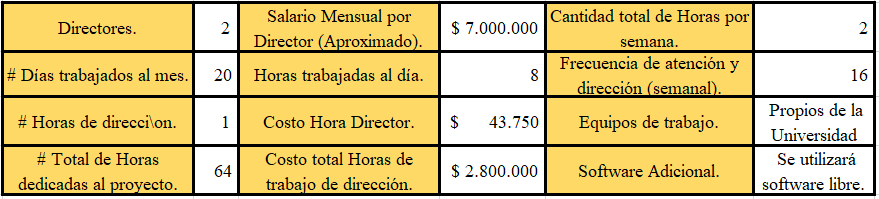
\includegraphics[scale=0.8]{img/considPUJ.png}
%%%		\end{center}
%%%		\caption{Consideraciones del proyecto respecto a la universidad. \label{tabconsidPUJ}}	
%%%	\end{table}
	
	\item Consideraciones del proyecto respecto al estudiante visto en el cuadro \ref{tabconsidYo}:
	
\begin{table}[H]
\centering
\scalebox{0.7}{
{\setlength{\arrayrulewidth}{0.8mm}
\begin{tabular}{ | >{\columncolor{tabla2}} p{3cm} | p{1.2cm} | >{\columncolor{tabla2}} p{3.5cm} | p{2.2cm} | >{\columncolor{tabla2}} p{4cm} | p{2.5cm} | }
\hline
{\bf\centering \bfseries\small Estudiante(s)} & {\bf\centering  1} & {\bf\centering \bfseries\small Salario Mensual por Estudiante \\ (Aproximado).}
 & {\bf\centering \bfseries\small \$ 1'.300.000} & {\bf\centering \bfseries\small Cantidad total de horas por  semana} & {\bf\centering  60}\\ \hline
{\bf\centering \bfseries\small  \# Total de Horas dedicadas al proyecto} & {\bf\centering 600} & {\bf\centering \bfseries\small \# Horas trabajadas al día} & {\bf\centering   10}
 & {\bf\centering \bfseries\small  \# Total de semanas trabajadas} & {\bf\centering  10}\\ \hline
 {\bf\centering \bfseries\small  \# Costo hora Estudiante} & {\bf\centering \$ 5.417} & {\bf\centering \bfseries\small Costo total Horas de trabajo dedicadas al proyecto} & {\bf \bfseries\small \$ 4'.160.000} & {\bf\centering \bfseries\small Equipos, Software y material de trabajo adicional} & {\bf\centering  Propios del estudiante} \\ \hline
\end{tabular}}}
		\caption{Consideraciones del proyecto respecto al estudiante. \label{tabconsidYo}}
\end{table}		
	
	
	
%	\begin{table}[H]
%		\begin{center}
%			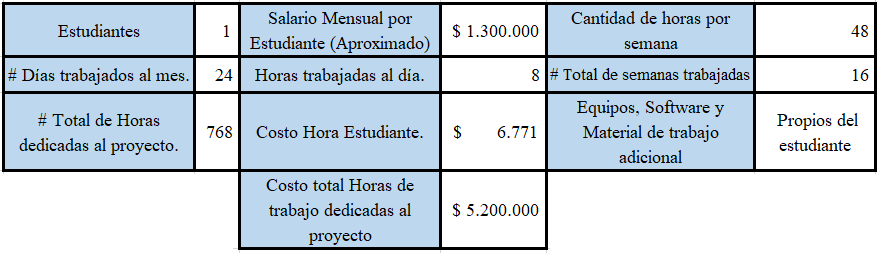
\includegraphics[scale=0.8]{img/considYo.png}
%		\end{center}
%		\caption{Consideraciones del proyecto respecto al estudiante. \label{tabconsidYo}}
%	\end{table}

\end{itemize}       


\subsubsection{Presupuesto}
El presupuesto del proyecto se observa en el Cuadro \ref{tabpresupuesto}.%
%	

%%%\begin{table}[H]
%%%\centering
%%%\scalebox{0.7}{
%%%{\setlength{\arrayrulewidth}{0.8mm}
%%%\begin{tabular}{ | p{1cm} | p{3cm} | p{5cm} |  p{2.5cm} | p{3.5cm} | p{3cm} | }
%%%\hline
%%%\begin{sideways}\multirow{5}{*}{UNIVERSIDAD}\end{sideways} & \multicolumn{1}{|>{\columncolor{blue2}}|}{CONCEPTO} & \multicolumn{1}{|>{\columncolor{blue2}}|}{REFERENCIA} & \multicolumn{1}{|>{\columncolor{blue2}}|}{CANT.} & \multicolumn{1}{|>{\columncolor{blue2}}|}{\$/Unidad} & \multicolumn{1}{|>{\columncolor{blue2}}|}{SUB TOTAL}\\ 
%%%\cline{2-6}
%%% & \multicolumn{1}{|>{\columncolor{tabla2}}|}{Costos dirección de trabajo de grado} & \multicolumn{1}{|>{\columncolor{beige}}|}{Asesoría y dirección del trabajo de grado del estudiante} & \multicolumn{1}{|>{\columncolor{beige}}|}{1} & \multicolumn{1}{|>{\columncolor{beige}}|}{\$ 546.875} & \multicolumn{1}{|>{\columncolor{beige}}|}{\$ 546.875}\\
%%%\cline{2-6}
%%% & \multicolumn{1}{|>{\columncolor{tabla2}}|}{Seguridad social y costos adicionales} & \multicolumn{1}{|>{\columncolor{beige}}|}{Costos adicionales por contratación de personal del proyecto} & \multicolumn{1}{|>{\columncolor{beige}}|}{1} & \multicolumn{1}{|>{\columncolor{beige}}|}{\$ 109.375} & \multicolumn{1}{|>{\columncolor{beige}}|}{\$ 109.375}\\
%%%\cline{2-6}
%%% & \multicolumn{1}{|>{\columncolor{tabla2}}|}{Equipos o instrumentación adicional} & \multicolumn{1}{|>{\columncolor{beige}}|}{Costo aproximado de sensores, elementos, herramientas, servicios y material de trabajo} & \multicolumn{1}{|>{\columncolor{beige}}|}{1} & \multicolumn{1}{|>{\columncolor{beige}}|}{\$ 2'.000.000} & \multicolumn{1}{|>{\columncolor{beige}}|}{\$ 2'000.000}\\
%%%\cline{2-6}
%%%%
%%%%
%%% & \multicolumn{4}{|>{\columncolor{lightgreen}}|}{SUBTOTAL} & \multicolumn{1}{|>{\columncolor{lightgreen}}|}{\$ 2'.656.250}\\
%%%\hline
%%%%
%%%%\begin{sideways}\multirow{5}{|>{\columncolor{darkgreen}}c|}{Estudiante}\end{sideways} & \multicolumn{1}{|>{\columncolor{blue2}}c|}{Concepto} & \multicolumn{1}{|>{\columncolor{blue2}}c|}{Referencia} & \multicolumn{1}{|>{\columncolor{blue2}}c|}{Cant.} & \multicolumn{1}{|>{\columncolor{blue2}}c|}{\$\/Unidad} & \multicolumn{1}{|>{\columncolor{blue2}}c|}{Subtotal 1}\\
%%%%%\cline{}
%%%%& & \multicolumn{1}{|>{\columncolor{tabla2}}c|}{Costos de trabajo por estudiante practicante} & \multicolumn{1}{|>{\columncolor{beige}}c|}{Investigación, Mano de obra y desarrollo del trabajo de grado del estudiante} & \multicolumn{1}{|>{\columncolor{beige}}c|}{1} & \multicolumn{1}{|>{\columncolor{beige}}c|}{3'.250.000} & \multicolumn{1}{|>{\columncolor{beige}}c|}{3'.250.000}\\
%%%%& & \multicolumn{1}{|>{\columncolor{tabla2}}c|}{Seguridad social y costos adicionales} & \multicolumn{1}{|>{\columncolor{beige}}c|}{Costos adicionales por contratación de personal estudiantil del proyecto} & \multicolumn{1}{|>{\columncolor{beige}}c|}{1} & \multicolumn{1}{|>{\columncolor{beige}}c|}{650.000} & \multicolumn{1}{|>{\columncolor{beige}}c|}{650.000}\\
%%%%& & \multicolumn{1}{|>{\columncolor{tabla2}}c|}{Equipos o instrumentación adicional} & \multicolumn{1}{|>{\columncolor{beige}}c|}{Costo aproximado de sensores, elementos, servicios, software y\/o material de trabajo} & \multicolumn{1}{|>{\columncolor{beige}}c|}{1} & \multicolumn{1}{|>{\columncolor{beige}}c|}{1'.000.000} & \multicolumn{1}{|>{\columncolor{beige}}c|}{1'.000.000}\\
%%%%
%%%%& & \multicolumn{4}{|>{\columncolor{lightgreen}}c|}{SUBTOTAL} & \multicolumn{1}{|>{\columncolor{lightgreen}}c|}{4'.900.000}\\
%%%%
%%%%\multicolumn{5}{|>{\columncolor{darkgreen}}c|}{COSTOS TOTALES} & \multicolumn{1}{|>{\columncolor{darkgreen}}c|}{7'.556.250}
%%%
%%%\end{tabular}}}
%%%		\caption{Presupuesto del proyecto. \label{tabconsidYo}}
%%%\end{table}		
%%%	


%%\begin{tabular}{|l|l|l|l|}\hline
%%  %\multirow{5}{*}{numeric literals} & \multirow{5}{*}{integers} & in decimal & \verb|8743| \\ \cline{3-4}
%%  \multirow{5}{*}{UNIVERSIDAD} & \multicolumn{1}{|l|}{CONCEPTO} & \multicolumn{1}{|l|}{REFERENCIA} & \multicolumn{1}{|l|}{CANT.} & \multicolumn{1}{|l|}{\$/Unidad} & \multicolumn{1}{|l|}{SUB TOTAL}\\
%%  & & \multirow{2}{*}{in octal} & \verb|0o7464| \\ \cline{4-4}
%%  & & & \verb|0O103| \\ \cline{3-4}
%%  & & \multirow{2}{*}{in hexadecimal} & \verb|0x5A0FF| \\ \cline{4-4}
%%  & & & \verb|0xE0F2| \\ \cline{2-4}
%%  & \multirow{5}{*}{fractionals} & \multirow{5}{*}{in decimal} & \verb|140.58| \\ \cline{4-4}
%%  & & & \verb|8.04e7| \\ \cline{4-4}
%%  & & & \verb|0.347E+12| \\ \cline{4-4}
%%  & & & \verb|5.47E-12| \\ \cline{4-4}
%%  & & & \verb|47e22| \\ \cline{1-4}
%%  \multicolumn{3}{|l|}{\multirow{3}{*}{char literals}} & \verb|'H'| \\ \cline{4-4}
%%  \multicolumn{3}{|l|}{} & \verb|'\n'| \\ \cline{4-4}          %% here
%%  \multicolumn{3}{|l|}{} & \verb|'\x65'| \\ \cline{1-4}        %% here
%%  \multicolumn{3}{|l|}{\multirow{2}{*}{string literals}} & \verb|"bom dia"| \\ \cline{4-4}
%%  \multicolumn{3}{|l|}{} & \verb|"ouro preto\nmg"| \\ \cline{1-4}          %% here
%%\end{tabular}



	\begin{table}[H]
		\begin{center}
			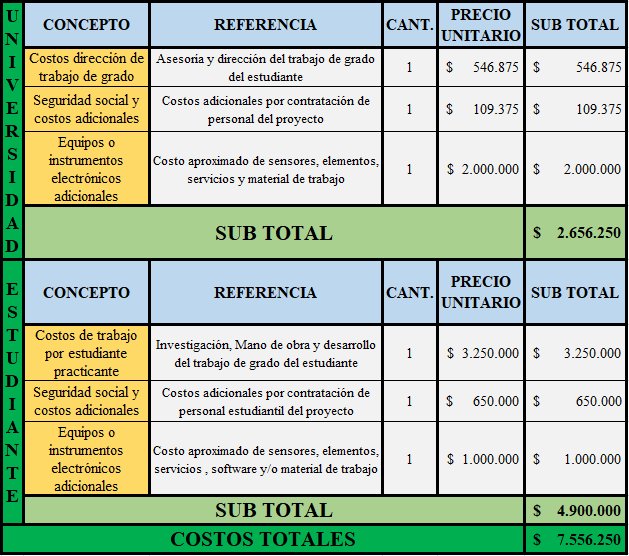
\includegraphics[scale=0.9]{img/presuTot3.png}
		\end{center}
		\caption{Presupuesto del proyecto. \label{tabpresupuesto}}
	\end{table}

 
